%\documentclass[defaultstyle,10pt,Helvetica,oneside]{istulthesis}
\documentclass[defaultstyle,10pt,Helvetica,twoside,openright]{resources/istutlthesis}

\input{resources/preamble}

\begin{document}

\ifnum 1>0
\newcommand{\pd}[1]{\textit{\textcolor{red}{[Peter]: #1}}}
\newcommand{\bsd}[1]{\textit{\textcolor{red}{[Baltasar]: #1}}}
\newcommand{\rr}[1]{\textit{\textcolor{red}{[Rodrigo]: #1}}}
\definecolor{aoe}{rgb}{0.0, 0.5, 0.0}
\newcommand{\update}[1]{{\color{aoe}#1}}
\newcommand{\new}[1]{{\color{blue}#1}}
\else
\newcommand{\pd}[1]{}
\newcommand{\bsd}[1]{}
\newcommand{\rr}[1]{}
\newcommand{\update}[1]{}
\newcommand{\new}[1]{}
\fi

\pdfbookmark[0]{Titlepage}{Title}
% #############################################################################
% DEFINE THE Front Cover Page of Thesis-MSc
% !TEX root = ./main.tex
% #############################################################################
% Thesis-MSc
% Version 4, August 2022
% BY: Prof. Rui Santos Cruz, rui.s.cruz@tecnico.ulisboa.pt
% #############################################################################
%
% REQUIRED LOGO:
% The university logo image: arguments correspond to {left}{top} position.
% IST rules determine the position to be be 2cm from top, left page edge
\univlogo{20mm}{20mm}{img/ist_logo}
% OPTIONAL IMAGE:
% The thesis image: arguments are the start position in the page.
% You can change the image for your thesis, replacing the image name.
% If no image is desired, just comment the command
\thesislogo{25mm}{50mm}{img/thesis_logo}
%
% -----------------------------------------------------------------------------
% REQUIRED: Thesis TITLE
\title{Restart-Rollback: A Fault model for distributed systems
with persistent state}
% OPTIONAL: Thesis SUBTITLE
\subtitle{}
%
% -----------------------------------------------------------------------------
% REQUIRED: Author
% Author full Name
\author{Baltasar Azevedo e Silva Dinis}
%
% -----------------------------------------------------------------------------
% The official name of the course/degree. Please chose portuguese or english
% un-comment the line corresponding to your degree.
% You can add a degree name using thie following construct:
%
\degree{Information Systems and Computer Engineering}
%\degree{Engenharia Informática e de Computadores}
%\degree{Telecommunications and Informatics Engineering}
%\degree{Engenharia de Telecomunicações e Informática}
%
% -----------------------------------------------------------------------------
% REQUIRED: The SUPERVISOR(s) - maximum of two
\supervisor{Prof. Rodrigo Rodrigues}
% If no co-Supervisor comment the next line
\othersupervisor{Prof. Peter Druschel}
%
% -----------------------------------------------------------------------------
% REQUIRED: Date of examination
% Insert the Date of the Thesis discussion (format is MONTH and YEAR)
\date{November 2022}
%
% -----------------------------------------------------------------------------
% The following command define the author colors for Tracking Changes in doc in case you use Tracking
% the Two letters identify each author
\definechangesauthor[color=forestgreen]{MN}
\definechangesauthor[color=blue]{JO}
\definechangesauthor[color=red]{PT}

% -----------------------------------------------------------------------------
% Select 'false' when delivering the draft version of the thesis.
% The committee members should not be printed for the draft version.
% Select 'true' after the Examination Committee has accepted the thesis as final
\finalthesis{true}
%\finalthesis{false}
%
% -----------------------------------------------------------------------------
% The members of the Examination Committee
% Normally there is only the "vogalone"
% Comment the other if not necessary
\chairperson{TBD}
\vogalone{Prof. Nuno Santos}
%\vogaltwo{Dr. Name of Second Committee Member}
%\vogalthree{Eng. Name of Third Committee Member}
%
% -----------------------------------------------------------------------------
% The second page should be white with the Copyright message.

\maketitle
\thispagestyle{empty}
\cleardoublepage{}

\setcounter{page}{1} \pagenumbering{roman}
\baselineskip 18pt  % line spacing: -12pt for single spacing
                   %               -18pt for 1 1/2 spacing
                   %               -24pt for double spacing
\pdfbookmark[0]{Acknowledgments}{acknowledgments}
\begin{acknowledgments}
	% #############################################################################
% Agradecimentos / Acknowledgments
% !TEX root = ../main.tex
% #############################################################################

\noindent I would like to thank Professor Rodrigo
Rodrigues, not only for his supervision of this thesis but for
over four years of mentoring and countless doors he has opened for me.
Without a doubt, my academic, professional and
personal development would not have been the same without his
intervention. I would also like to thank Professor Peter
Druschel, who welcomed me multiple times at the Max Planck
Institute for Software Systems in Saarbrücken, an institution
where I learned a lot of lessons which I will carry with me and
for his astute comments and scientific rigour, from which I have
learned a lot.

I would like to acknowledge several other colleagues, mentors and
contributors, who have been with me through my
academic journey: Afonso Tinoco, Roberta De Viti, Professor
Deepak Garg, Professor Vijay Chidambaram, Professor Bobby
Bhattacharjee and Professor Pedro Adão.

I would like to thank my parents, for the housing and food they
have provided me through the years, an indispensible prerequisite for good
research. Also, for raising me.

Finally, I would like to thank my friends. Although words are not
nearly enough to describe the shared moments (both of joy and
hardship), the companionship, the comraderie and the bond that
connects us, I am forever grateful: Afonso, Andreia, Chico,
Cintrão, Donga, Filipa, Gaspar, Homem, João, Lamego, Lé, Maria, Mariana, Marta Ambrósio,
Marta Sousa, Pacheco, Pedro, Pina, Regouga, Reynolds, Rocha,
Sanches, Vasco, Zé e Leonor.

\end{acknowledgments}

\begin{abstract}
	% #############################################################################
% Abstract Text
% !TEX root = ../main.tex
% #############################################################################
% reset acronyms
\acresetall
% use \noindent in firts paragraph

\vskip -.5cm
\noindent \acsp{TEE} ensure the confidentiality and integrity of
computations in hardware. Subject to the \acs{TEE}'s threat model,
the hardware shields computation from most externally induced
faults except crashes. As a result, \acs{CFT}
replication protocols should be sufficient when replicating
\acsp{TEE}. However, \acsp{TEE} do not offer
efficient means of ensuring the freshness of persistent state,
which can be rolled back to an earlier version. In this
dissertation, we propose the \ac{RR} fault model for replicating
\acsp{TEE}, which precisely captures the possible fault behaviors
of \acsp{TEE} with external state, making it possible to avoid
using expensive \acs{BFT} protocols. Then, we show that existing
\acs{CFT} replication protocols can be easily adapted to this fault model
with few changes, while retaining their original performance.
\vskip 0cm
To illustrate the usefulness of \acs{TEE} replication under
\acs{RR}, we built a replicated metadata service called
\acs{TEEMS}, which can be used to add \acs{TEE}-grade
confidentiality, integrity, and freshness to untrusted cloud
storage. Then, we showcase the generality of the \acs{RR} model,
by applying it to the context of replicated \acsp{KVS}. Current
replicated \acsp{KVS} make a tradeoff between latency, throughput
and durability, depending on whether they flush writes before
replying (which offers poor performance) or batch writes in
memory (possibly losing data if nodes crash before flushing). We
observe that the latter case effectively constitutes a rollback,
which is captured by \acs{RR}.
\vskip 0cm
We implemented the various protocols and systems, and our
evaluation shows performance that is comparable to \acs{CFT}
systems but with stronger guarantees, and significantly better
than \acs{BFT} systems.

\end{abstract}

\begin{keywords}
	% #############################################################################
% English Keywords
% !TEX root = ../main.tex
% #############################################################################
% reset acronyms
\acresetall
% use \noindent in firts paragraph
\noindent
Cloud Storage,
Distributed Storage,
Distributed Systems,
Durability,
Fault Model,
Persistence,
Replication,
Replication Protocol,
Storage,
Trusted Execution Environments

\end{keywords}
\clearpage

\thispagestyle{empty}

\cleardoublepage{}

\begin{resumo}
    \vskip -1cm
	% #############################################################################
% RESUMO em Português
% !TEX root = ../main.tex
% #############################################################################
% use \noindent in firts paragraph
% reset acronyms
\acresetall
\noindent Ambientes de Execução Confiável (em inglês, TEEs)
garantem a confidencialidade e integridade de computações ao
nível do \textit{hardware}. Sobre o modelo adversarial dos TEEs, o
\textit{hardware} protege a computação da maioria das falhas
induzidas externamente, excepto falhas de \textit{crash}, em que
um TEE simplesmente vai abaixo (e.g., quando falta a
eletricidade). Contudo, TEEs, não possuem métodos eficientes de
garantir a frescura do seu estado persistente, que pode ser
revertido para uma versão anterior. Nesta dissertação, propomos o
modelo de faltas \ac{RR} para replicação de TEEs, que captura
exatamente os comportamentos de falta de TEEs com estado externo,
evitando a utilização de protocolos BFT, que incorrem num custo
superior. Mostramos que protocolos CFT existentes podem ser
adaptados facilmente para este modelo de faltas com poucas
alterações, mantendo a sua performance original.
\vskip -0cm
Para ilustrar a utilidade da replicação de TEEs segundo o
modelo RR, construímos um serviço de metadados replicado chamado
TEEMS, que pode ser usado para acrescentar confidencialidade,
integridade e frescura a armazenamento em cloud ao nível das
proteções dos TEEs. Seguidamente, exemplificamos a generalidade
do modelo RR, aplicando-o ao contexto de KVSs replicadas. KVSs
replicadas atuais escolhem entre latência, \textit{throughput} e
durabilidade, dependendo se sincronizam as escritas antes de
responderem aos pedidos (o que oferece uma \textit{performance}
fraca) ou se combinam várias escritas numa \textit{batch} em
memória (possivelmente perdendo dados se os nós forem abaixo
antes da escrita ser sincronizada). Observamos que o último
caso effetivamente corresponde a uma reversão de estado, que é
capturada pelo modelo RR.
\vskip 0cm
Impelmentámos os vários protocolos e sistemas, e a nossa
avaliação demonstra que a \textit{performance} é comparável à de
sistemas CFT mas com garantias mais fortes e significativamente
superior à de sistemas BFT.

\end{resumo}
    \vskip -1cm
\begin{palavraschave}
    \vskip -1cm
	% #############################################################################
% Portuguese Keywords
% !TEX root = ../main.tex
% #############################################################################
% reset acronyms
\acresetall
% use \noindent in firts paragraph

\noindent TODO

\end{palavraschave}
\clearpage

\thispagestyle{empty}

% This is required for the Fancy Chapters with minitoc
\dominitoc{}
\dominilof{}
\dominilot{}

\renewcommand{\baselinestretch}{1}
\pdfbookmark[0]{Contents}{toc}
\tableofcontents
\cleardoublepage{}

% reposition baseline
\renewcommand{\baselinestretch}{1.5}

\pdfbookmark[1]{List of Figures}{lof}
\listoffigures
\cleardoublepage{}
\begingroup
    % \let\clearpage\relax
    % \let\cleardoublepage\relax
    % \let\cleardoublepage\relax
% List of Tables
\pdfbookmark[1]{List of Tables}{lot}
\listoftables
\cleardoublepage{}

%\pdfbookmark[1]{List of Algorithms}{loa}
%\listofalgorithms{}
%\endgroup
%\cleardoublepage{}

%\pdfbookmark[1]{Listings}{lol}
%\lstlistoflistings{}
%\cleardoublepage{}
% -----------------------------------------------------------------------------
% % List of acronyms
\pdfbookmark[1]{Acronyms}{loac}
\chapter*{\tlangAcronyms}
% #############################################################################
% This is the ACRONYMS Definition
% !TEX root = ../main.tex
% #############################################################################
% Do not forget to reorder Alphabetically the ACRONYMS !!!
% If there are special cases for Plural form see example hereunder
\begin{acronym}[H.264/SVC]
    \acro{ABD}{Attiya, Bar-Noy, Dolev}
	\acro{BFT}{Byzantine Fault Tolerant}
	\acro{CFT}{Byzantine Fault Tolerant}
	\acro{R2-S2}{Restart-Rollback Storage System}
	\acro{RR}{Restart-Rollback}
    \acro{SMR}{state machine replication}
	\acro{TEE}{Trusted Execution Environment}
	\acro{TEEMS}{TEE Metadata System}
    \acro{YCSB}{Yahoo! Cloud Serving Benchmark}
\end{acronym}

\clearpage
\cleardoublepage{}
% -----------------------------------------------------------------------------

\setcounter{page}{1} \pagenumbering{arabic}
\baselineskip 18pt
% -----------------------------------------------------------------------------

\acresetall{}
\fancychapter{Introduction}\label{chap:intro}
\cleardoublepage{}

\bsd{\begin{enumerate}
    \item State of the Art: replicated systems with persistent
        state are treated akin to volatile state replicated
        systems, with the additional option of a node recovering
        from local state after restart;
    \item In certain security sensitive contexts, namely TEEs.
        this does not work. Nodes have limited control over
        persistent state, especially across restarts.
    \item To recover safely from persistent state one must use a
        stronger fault model. Currently, the only adequate model
        is BFT. This is far too strong, considering that nodes
        have correct and trusted execution.
    \item To bridge this gap, we develop the RR model, where
        a node's persistent state can be rolled back to a
        previous valid version. This way, TEEs can recover from
        their local persistent state.
    \item Taking a step back, this can be useful to extract
        performance from other replicated systems. In particular,
        by being more relaxed with syncronizing the volatile
        and persistent states, we can batch more aggressively.
        This would be otherwise unsafe, as a crash could rollback
        a replica.
    \item To evaluate our approach, we developed two systems,
        TEEMS and R2-S2. (Description of the systems and
        experimental results)
\end{enumerate}}

Replication is a standard technique in distributed systems, which adds
fault tolerance to a service implemented by an individual networked
node. To ensure that the replicated service appears to clients like
its single-node equivalent except for higher availability, a
replication protocol coordinates the replicated
nodes. For instance, to replicate a key value store \new{(i.e.:
a storage system which offers a simple get/put interface)} one can use the \ac{ABD}~\cite{abd}
protocol. For more complex applications that can be modelled
using a deterministic state machine, an \ac{SMR} protocol like
Paxos~\cite{paxos} may be used.

\new{Durability, i.e.\ not losing data even in the event of faults, is a key property of storage
systems. For replicated storage systems, adding local persistency
to the nodes that make up the system is a common practice. This
allows replicas to recover from crashes (in which they lose their
volatile state)} from their local \new{persistent} state, which in turn makes the
system resilient to catastrophic full system
shutdowns~\cite{bolosky:paxos}. From a
formal point of view, however, these systems are commonly treated in a
very similar fashion to others that store their state solely in
volatile memory. Indeed, when the persistent aspect of nodes
is explicitely considered, protocols are almost identical, with
small extensions that describe when and what data nodes need to
persist so that, in the event of a restart, the node can
operate as if nothing happened.

\new{This lack of explicit consideration of the persistent state
becomes a problem in certain security sensitive cases, in
particular in the context of \acp{TEE}. \acp{TEE} are
applications running in a special hardware-protected environment,
where the CPU shields the application, guaranteeing the integrity
and confidentiality of the code execution and the associated
volatile memory, in a way that it can be remotely attested that
the hardware protections were correctly set up. As such, they
have become an attractive solution for system administrators who
make deployments in infrastructure that they do not directly
control (e.g.\ the public cloud). \acp{TEE} run in an highly
adversarial attacker model, where the owner and operator of the
hardware is not trusted, and as such their control over the
persistent storage is quite limited, especially in the event of a
restart, where the \ac{TEE} cannot maintain records that ensure
the integrity and freshness of the persistent storage it is
using. Simply applying current replicated protocols would pose a
correctness and security problem.}\bsd{is this too vague? it is developed further down}

Despite these challenges, networked services implemented inside \acp{TEE} like
ARM TrustZone~\cite{armTZ}, AMD SEV-SNP~\cite{amdsev,
amdsev-snp}, Intel SGX~\cite{intelsgx}, or the future Intel
TDX~\cite{inteltdx} and ARM CCA~\cite{arm-cca} can similarly
benefit from replication.  Replicated \ac{TEE}-based systems aim
to combine the confidentiality, integrity, and remote attestation
of \acp{TEE} with replication to ensure high availability.
Examples include permissioned blockchains~\cite{teechain},
monotonic counters for ensuring state freshness~\cite{rote},
in-memory key-value stores~\cite{avocado-atc21}, as well as
broadcast and common random number generator
primitives~\cite{p2p-sgx}.

A key design decision in all replicated systems is the choice of fault
model underlying the replication protocol. This model captures the set
of faults that can affect an individual replica.  For instance, in the
{\em crash-fault model}, faulty nodes are assumed to execute correctly
until they crash at an arbitrary point in their execution, when they
seize to perform further steps until they restart. In the {\em
  Byzantine fault model}, faulty nodes may perform arbitrary
actions. The choice of fault model affects the complexity, overhead,
and tolerance threshold of a replication protocol, and is important
for both performance and security. A fault model that is too
pessimistic may lead to unnecessary safeguards, which can impact both
performance and the cost of replication. Conversely, a fault model
that is too optimistic may fail to account for all faults that can
occur, which then leads to broken assumptions and loss of correctness
or security of the replicated system.

In the case of \ac{TEE}-based replication, the choice of existing systems
that store replica state persistently~\cite{teechain,rote} was to
employ \ac{BFT} replication. This may seem
necessary given that rollback of persistent state is a behavior not
covered by the crash-fault model.  However, the Byzantine model is
much stronger than necessary for this setting. Intuitively, this
is because it assumes arbitrary behavior of
faulty components, thus not taking into account the integrity
guarantees for the code running inside \acp{TEE}.

To fill this gap in distributed replication research, we
introduce the \ac{RR} fault model, which
%is designed for replicated \ac{TEE}-isolated services and
captures precisely the set of faults that \acp{TEE} can suffer according to
their specification.  The main insight behind \ac{RR} is that,
apart from crash faults, whenever a \ac{TEE} restarts, the fault model
allows for a rollback of externally stored state to an earlier
version.  Such rollback events are possible because \acp{TEE} lack general
and high-performance means of ensuring the freshness of externally
stored state.  During an execution, however, the integrity of the
internal, volatile state of a \ac{TEE} is ensured by hardware, and the
integrity of any externally stored state can be ensured by standard
cryptographic means.

The \ac{RR} fault model occupies a middle ground between \ac{CFT}
and \ac{BFT}. As we will show, unlike CFT it provides
security for replicated \acp{TEE} by tolerating state roll-back at a cost
that is similar to \ac{CFT} and better than \ac{BFT}. Specifically, it is able
to substantially reduce the required communication, particularly for
read operations, in the common case where restarts are
infrequent.

Stepping back, we make the observation that the \ac{RR} fault
model can be useful, albeit for different reasons, in the more
general case of persistent replicated systems within the crash
model. A key factor for performance in this systems are the slow
accesses to untrusted storage, which must occur in the critical
path to ensure the correctness of the system. By batching
multiple requests together, it is possible to reduce this
overhead, increasing throughput at the expense of the additional
latency required to form the batch. Leveraging the \ac{RR} model,
it is possible to form batches more aggressively, replying to
certain requests before synchronizing to persistent storage. This
would otherwise be unsafe, as a crash before the synchronization
would constitute an effective rollback, which the \ac{RR} model
captures.

To demonstrate the potential of the \ac{RR} model, we apply it to
two types of replication protocols, namely the \ac{ABD}
 read/write replication protocol and the Paxos \ac{SMR}
protocol, showing that this adaptation is relatively straightforward.
We then use these protocols to devise two systems: \ac{TEEMS} and
\ac{R2-S2}. \ac{TEEMS}, a replicated metadata service,
is a relevant contribution in its own right, since
it enables Cloud storage with the same strong confidentiality and
integrity guarantees provided by \acp{TEE}. while also ensuring freshness
of data. \ac{TEEMS} is used with one or more untrusted cloud storage
services. \ac{TEEMS} maintains metadata for each data item (including the
encryption key, authentication code, latest version number and
policy), while ensuring strong security and enabling concurrent
sharing of data. \ac{R2-S2} is a replicated key value store built
using regular nodes (i.e. without TEEs or other security
mechanisms) that leverages the \ac{RR} model with the objective
of extracting higher throughput while retaining the strong reliability expected of a persistent
replicated system.

\section{Contributions}

In the \ac{TEE} context, we implemented the read/write
register and the \ac{SMR} protocols in three fault models:
\ac{CFT}, \ac{RR} and \ac{BFT}, and a prototype for \ac{TEEMS},
all using Intel SGX. In the storage context, we implemented
\ac{R2-S2} as a replication layer on top of a single node key
value store. We evaluated our prototypes using both
microbenchmarks and real-world workloads, namely
\ac{YCSB}~\cite{ycsb}.

Our contributions include:
\begin{enumerate}
    \item The \ac{RR} fault model, which is the first to capture
        precisely the fault behavior of \acp{TEE} that rely on external storage;
    \item A derivation of quorum sizes for replication protocols
        in the \ac{RR} model;
    \item Principles for the adaptation of \ac{CFT} protocols to
        the \ac{RR} model;
    \item Two protocols for this model, implementing read-write
        storage and \ac{SMR};
    \item The \ac{TEEMS} generic metadata service, and its integration with
        untrusted cloud storage services to give clients the ability to share
        and concurrently access persistent data with strong confidentiality,
        integrity, and freshness;
    \item The \ac{R2-S2} distributed key value store, which
        enables higher throughput from key value stores backed by
        persistent state;
    \item An extensive experimental evaluation of our protocols
        in the \ac{TEE} setting, with a \update{detailed} comparison with
        unsafe \ac{CFT} and expensive \ac{BFT} solutions;
    \item An experimental evaluation of the \ac{R2-S2}
        system.
\end{enumerate}


% #############################################################################
\section{Organization of the Document}

The rest of the thesis is organized as follows:
\Cref{chap:related} covers related work. In \cref{chap:model} we
formalize the \ac{RR} model and show the derivation of
\ac{RR}-based quorum systems and protocols. \Cref{chap:tee}
describes the usage of \acp{TEE} with \ac{RR}, with the
accompanying design and evaluation of \ac{TEEMS}. In
\cref{chap:storage} we present the design of
\ac{R2-S2} and its experimental evaluation.
\Cref{chap:conclusion} summarizes our work and presents possible
avenues for future work.

% #############################################################################

\if 0 % paper intro

Replication is a standard technique in distributed systems, which adds
fault tolerance to a service implemented by an individual networked
node. To ensure that the replicated service appears to clients like
its single-node equivalent except for higher availability, a
replication protocol coordinates the replicated
nodes. For instance, a state machine replication (SMR) protocol like
Paxos~\cite{paxos} may be used for this purpose.

Networked services implemented inside a trusted execution environment
(TEE) like ARM TrustZone~\cite{armTZ}, AMD SEV-SNP~\cite{amdsev,
  amdsev-snp}, Intel SGX~\cite{intelsgx}, or the future Intel
TDX~\cite{inteltdx} and ARM CCA~\cite{arm-cca} can similarly benefit
from replication.  Replicated \ac{TEE}-based systems aim to combine the
confidentiality, integrity, and remote attestation of \acp{TEE} with
replication to ensure high availability.
%and resilience to rollback attacks that revert the externally stored,
%persistent state of a TEE~\cite{memoir}
%\bsd{the reference to rollback attacks early on seems out of place,
%  since this is a gap in most replicated \acp{TEE}. Moreover, memoir is not
%  a replicated \ac{TEE} system}.
Examples include permissioned blockchains~\cite{teechain}, monotonic
counters for ensuring state freshness~\cite{rote}, in-memory key-value
stores~\cite{avocado-atc21}, as well as broadcast and common random
number generator primitives~\cite{p2p-sgx}.

A key design decision in all replicated systems is the choice of fault
model underlying the replication protocol. This model captures the set
of faults that can affect an individual replica.  For instance, in the
{\em crash-fault model}, faulty nodes are assumed to execute correctly
until they crash at an arbitrary point in their execution, when they
seize to perform further steps until they restart. In the {\em
  Byzantine fault model}, faulty nodes may perform arbitrary
actions. The choice of fault model affects the complexity, overhead,
and tolerance threshold of a replication protocol, and is important
for both performance and security. A fault model that is too
pessimistic may lead to unnecessary safeguards, which can impact both
performance and the cost of replication. Conversely, a fault model
that is too optimistic may fail to account for all faults that can
occur, which then leads to broken assumptions and loss of correctness
or security of the replicated system.

In the case of \ac{TEE}-based replication, the choice of existing systems
that store replica state persistently~\cite{teechain,rote} was to
employ Byzantine fault tolerant (BFT) replication. This may seem
necessary given that rollback of persistent state is a behavior not
covered by the crash-fault model.  However, the Byzantine model is
much stronger than necessary for this setting. Intuitively, this
is because it assumes arbitrary behavior of
faulty components, thus not taking into account the integrity
guarantees for the code running inside \acp{TEE}.

In this paper, we fill a gap in distributed replication research by
introducing the restart-rollback (\faultmodel) fault model, which
%is designed for replicated \ac{TEE}-isolated services and
captures precisely the set of faults that \acp{TEE} can suffer according to
their specification.  The main insight behind \faultmodel\ is that,
apart from crash faults, whenever a \ac{TEE} restarts, the fault model
allows for a rollback of externally stored state to an earlier
version.  Such rollback events are possible because \acp{TEE} lack general
and high-performance means of ensuring the freshness of externally
stored state.  During an execution, however, the integrity of the
internal, volatile state of a \ac{TEE} is ensured by hardware, and the
integrity of any externally stored state can be ensured by standard
cryptographic means.

The \faultmodel\ fault model occupies a middle ground between crash
fault tolerance (CFT) and BFT. As we will show, unlike CFT it provides
security for replicated \acp{TEE} by tolerating state roll-back at a cost
that is similar to CFT and better than BFT. Specifically, it is able
to substantially reduce the required communication, particularly for
read operations, in the common case where restarts are
infrequent.

To demonstrate the potential of the \faultmodel\ model, we apply it to
two types of replication protocols, namely the Attiya, Bar-Noy, Dolev
(ABD) read/write replication protocol and the Paxos
state machine replication (SMR)
protocol, showing that this adaptation is relatively straightforward.
%; and, we apply each protocol to a specific application scenario.
We then use these protocols to devise a replicated metadata service
called \sys, which is a relevant contribution in its own right, since
it enables Cloud storage with the same strong confidentiality and
integrity guarantees provided by \acp{TEE}. while also ensuring freshness
of data.
% and the ability to securely share data between clients by
% enforcing access policies. To this end, \sys\ provides a
% generic, scalable,
%\sys\ is a trustworthy metadata service hosted in a replicated set of
%TEEs, which may themselves be hosted by a diverse set of cloud
%providers for increased resilience.
%This service provides a semantically rich interface with
%persistent updates and read-modify-write (RMW) operations.
\sys\ is used with one or more untrusted cloud storage
services. \sys\ maintains metadata for each data item (including the
encryption key, authentication code, latest version number and
policy), while ensuring strong security and enabling concurrent
sharing of data.

%and updates this metadata and the respective data atomically using the simple read/write protocol for the \faultmodel\ model.\bsd{need to rewrite this, present that it uses both protocols}

%The second case study is inspired by permissioned blockchains, and
%their ability to improve performance by offloading transactions to a
%payment channel running a more efficient protocol, and then settling
%the final balance to the main blockchain. To support this, we built a
%state machine replication protocol based on the \faultmodel\ model,
%thus allowing the more complex operations of these payment channels to
%be supported in a resilient way.

We implemented both the read/write and SMR replication protocols for
three different fault models (\faultmodel, crash, and Byzantine), and
we also implemented \sys\ and used it to implement a new class of
secure cloud storage services. We evaluated the protocols using
microbenchmarks and the storage system using both microbenchmarks and
YCSB.  Our experimental results show that the protocols for the
\faultmodel\ model perform significantly better than their BFT
counterparts, and, compared to CFT, they perform identically while
additionally tolerating rollback attacks.
Furthermore, \sys\ offers secure, sharable storage at modest overhead.

Our contributions include:
%\begin{enumerate}
%\item
 (1) The \faultmodel\ fault model, which is the first to capture
precisely the fault behavior of \acp{TEE} that rely on external storage;
%    \item
(2) a derivation of quorum sizes for replication protocols in the
\faultmodel\ model;
      %     \item
(3) principles for the adaptation of CFT protocols to
the \faultmodel\ model;
%\item
(4) two protocols for this model, implementing read-write storage and
SMR;
        %    \item
(5) The \sys\ generic metadata service, and its integration with
untrusted cloud storage services to give clients the ability to share
and concurrently access persistent data with strong confidentiality,
integrity, and freshness;
%\item
(6) An extensive experimental evaluation of our protocol, and of the
storage solutions based on \sys\ in different deployment scenarios.
%\end{enumerate}


The remainder of the paper is organized as follows.  We motivate
our work and provide some background \S\ref{sec:fault_model},
describe the \faultmodel\ model in \S\ref{sec:model}, present the
replication protocols in the new model in
\S\ref{sec:protocol}, and an example application built using
those protocols in \S\ref{sec:metadata}.  We describe our
prototype implementations in \S\ref{sec:impl}, evaluate them
experimentally in \S\ref{sec:eval}, survey related work in
\S\ref{sec:related_work}, and conclude in \S\ref{sec:conclusion}.





\fi

\cleardoublepage{}

\fancychapter{Related Work}\label{chap:related}
\cleardoublepage{}

\cleardoublepage{}

\fancychapter{The \ac{RR} Fault Model}\label{chap:model}
\cleardoublepage{}

\cleardoublepage{}

\fancychapter{\ac{TEE} replication using the \ac{RR} model}\label{chap:tee}
\cleardoublepage{}

As we have discussed previously, \acp{TEE} are an interesting
option deploying replicated systems in an untrusted public cloud.
In this chapter, we present the \acf{TEEMS}, a replicated metadata
service for trusted cloud storage. \ac{TEEMS} has a double purpose in
the context of this dissertation: it showcases a practical system
using the \ac{RR} fault model and associated register and
\ac{SMR} protocols and provides the means of enhancing existing
cloud storage systems such that they can be trusted and remotely
attested in the same fault model as \acp{TEE} (and, by extension,
used by them as a persistent storage, with rollback protection).

This chapter is organized as follows.
Section~\ref{sec:teems_design}
provides the motivation and design of \ac{TEEMS}, followed by
Section~\ref{sec:teems_impl}, which describes the implementation
of \ac{TEEMS}. Finally, Section~\ref{sec:teems_eval} presents an
extensive evaluation of \ac{TEEMS} using real-world workloads
across different deployments.

\section{\ac{TEEMS}: Metadata service for trusted cloud
storage}\label{sec:teems_design}


\subsection{Motivation}

\acp{TEE} have enabled services like Azure Confidential
Computing~\cite{azure-conf} and Google Confidential
VMs~\cite{google-confVM}, where Cloud tenants can use compute
services without trusting the platform provider.  However, the
strong security properties from \acp{TEE} do not automatically
extend to cloud storage. To create a cloud-based system with
similar strong security guarantees of \acp{TEE}, it is only
natural to consider using \acp{TEE} as its building blocks. A
\ac{TEE}-encapsulated metadata service, replicated for
availability and fault-tolerance, can maintain encryption keys
and version information for data blobs stored in untrusted Cloud
storage.  By ensuring confidentiality, integrity, and freshness
of the metadata, the service extends the same guarantees to the
encrypted and versioned data blobs. Moreover, by supporting an
atomic update operation on metadata, the service enables
concurrent sharing of data blobs.

This approach needs to be integrated at the replication
level. Fundamentally, even assuming an efficient way for
storing the state of a single \ac{TEE}, this solution would still be
unable to support concurrent sharing between multiple \acp{TEE}. This
is because ensuring freshness of a single \ac{TEE}'s own state relies
on persistently storing a monotonic counter~\cite{ariadne,rote,ice}
or a top-level hash~\cite{memoir}, which can only be updated by
the \ac{TEE} itself.  Concurrent sharing of persistent state instead
requires atomic, concurrent updates of state blobs and their
associated metadata (e.g., counter).

We designed and implemented a replicated metadata service called
\ac{TEEMS} (for \ac{TEE}-based Metadata Service) based on the
\ac{RR} fault model. \ac{TEEMS}'s replicas can be hosted in a
diverse set of cloud providers for high availability and
resilience.
%
\ac{TEEMS} provides a read/write interface for metadata and guarantees that
readers always receive the metadata (e.g., encryption key) of the most
recent version of a data blob.  \ac{TEEMS} also supports access control
policies for metadata, and therefore allows clients to selectively
share the associated data blobs.  The service therefore enables
trusted storage services that extend the strong guarantees of today's
\ac{TEE}-based cloud compute services to persistent storage.

\subsection{\ac{TEE}-grade cloud storage with \ac{TEEMS}}

Clients can use \ac{TEEMS} to lend untrusted cloud storage \ac{TEE}-level
guarantees, by using the API in Table~\ref{tab:teems}.
\ac{TEEMS} maintains metadata for each data blob, i.e. a short summary of
the most recent version of a data blob, namely its hash and encryption
key. The encrypted data blob is then stored in an ordinary cloud
storage service. This extends the integrity, confidentiality,
freshness and selective concurrent sharing properties of the
metadata service to the cloud storage, while relying on the cloud
service only for storage and availability.

\begin{table}[!t]
    \centering
    \renewcommand{\arraystretch}{0.9} % this reduces the vertical spacing between rows
    \begin{small}
    \begin{tabular}{rll}
        \hline
        Return Value && {Command and Arguments}\\
        \hline
        \{\lArg{status}\} &\eq& {\sysC{teems-init}(\lArg{client ID})}\\
        \{\lArg{status}\} &\eq&{\sysC{teems-close}}()\\
        \{\lArg{status}\} &\eq&{\sysC{teems-write}}(\lArg{id}, \nArg{val})\\
        \{\lArg{status}, \nArg{val}, \lArg{ver}\} &\eq&{\sysC{teem-read}}(\lArg{id})\\
        \{\lArg{status}\} &\eq&{\sysC{teems-delete}}(\lArg{id})\\
        \{\lArg{status}\} &\eq&{\sysC{teems-change-policy}}(\lArg{id}, \lArg{policy-code})\\
        \hline
    \end{tabular}
    \end{small}
    \caption{\ac{TEEMS} Interface}\label{tab:teems}
\end{table}

Concurrent sharing of mutable data fundamentally requires a
read-modify-write operation (i.e., some form of \ac{SMR}).
However, state machine operations are more expensive than
read/write register operations. \ac{TEEMS} minimizes the use of
state machine operations in situations where writers typically
perform multiple updates of a data blob before other writers
perform an update as follows.  We mediate access to the metadata
via single writer policies, and implement policy changes via the
more expensive read-modify-write state machine operation. Simply
reading and updating the metadata of a blob (by the current
writer) is implemented using efficient distributed register
operations.  This approach ensures safe concurrent sharing of
data blobs while minimizing the more expensive policy changes to
cases when the writer for a blob changes. The full \ac{TEEMS}
interface is summarized in Table~\ref{tab:teems}.

Storage operations involve the following sequence of steps.  When an
operation to write a new data blob $d$ associated with id $i$ is
invoked, the client library starts by generating a symmetric
encryption key $k$. In our implementation, we use an authenticated
encryption scheme (AES-GCM), which generates a ciphertext ($\langle d
\rangle_k$) and a MAC ($MAC(d)$) of $d$.
%
The encrypted object and corresponding MAC are then stored in one
or more untrusted cloud storage services, under a randomly
created identifier $i_{store}$. Let $a$ be the access control
list for the newly stored data blob $d$. After the data has been
successfully written to untrusted storage, the library contacts
the \ac{TEEMS} metadata service to update the metadata for id $i$:
\[ \langle i,k,a,i_{store},MAC(d) \rangle   \]
%
The write operation concludes successfully after both the data
write and the metadata update complete. Finally, the library
deletes earlier versions of the blob from the data store.

When a read for id $i$ is invoked, the client library starts by
querying the \ac{TEEMS} service for the most recent version of
the metadata associated with the id $i$. After retrieving the
tuple $\langle i,k_i,i_{store},MAC(d_i) \rangle$, the client
library then uses the id $i_{store}$ to retrieve the encrypted
data from untrusted storage. This encrypted data $\langle
d'\rangle_{k_i}$ is read and then decrypted using $k_i$,
obtaining $d'$ and $MAC(d')$. Finally, its integrity  is
validated by comparing $MAC(d')$ and $MAC(d_i)$.

Finally, the access to the untrusted storage can be optimized by
employing caching at the client. We can either cache full blobs (to
avoid having to access the untrusted store) or name hints (for
enabling parallel access to the metadata service and the untrusted
store).  In either case, the metadata always has to be fetched and
compared with the cached or retrieved version, since only the
\ac{TEEMS} metadata service can ensure freshness of data blobs.

\subsection{Leveraging different storage protocols}

\ac{TEEMS} implements the metadata read/write operations efficiently using
our \ac{RR}-tolerant ABD protocol (Section~\ref{ssec:abd}).  However,
updating the policies stored by \ac{TEEMS} --- which enables concurrent
 sharing --- requires a read-modify-write operation, because changing
a policy requires reading the policy first to check if the client has
permission to modify it.  Therefore, policy changes are implemented
using the \ac{RR}-tolerant SMR protocol
(Section~\ref{ssec:paxos}).  This combination of protocols allows us
to achieve both efficient reads and writes in the normal case, and
concurrent write sharing via atomic policy changes through state
machine updates.

In this design, the state of our state machine is an epoch number
and an associated policy description. Crucially, the
epoch number is also readable by the read/write protocol. As
such, a policy change is a state machine operation which
evaluates the current policy, replacing it with the proposed
policy and incrementing the epoch number, if such permission is
granted. The epoch number increment is then immediately
visible to register operations.

\begin{figure}[t]
  \begin{small}
    \textbf{Write Metadata (key $k$, value $v$)}

    \begin{enumerate}[itemsep=0pt,parsep=0pt]

        \item \textbf{smr\_get\_policy ($k$)}

        \item \textbf{if} $eval(policy) == \textsc{access denied}$ \textbf{then}\\
            \tabto{.5cm}    \textbf{return} $\textsc{access denied}$

        \item \textbf{register\_write ($k$, $v$, $epoch$)}

        \item \textbf{if} $\textsc{epoch changed}$ \textbf{then}\\
            \tabto{.5cm}    \textbf{restart operation}

        \item \textbf{return} \textsc{Success}
    \end{enumerate}

  \end{small}
  \caption{Slow but trivially correct mixing of the protocols.
    The read operation is in all aspects similar.}\label{fig:teems_slow_correct}
\end{figure}

\begin{figure}[t]
  \begin{small}
    \textbf{Write Metadata (key $k$, value $v$)}

    \begin{enumerate}[itemsep=0pt,parsep=0pt]

        \item \textbf{smr\_optimized\_get\_policy ($k$)} in
            parallel with \textbf{register\_get\_version ($k$)}

        \item \textbf{if} $smr\_optimized\_get\_policy$ fails \textbf{then}\\
            \tabto{.5cm}    \textbf{fallback} to slow operation

        \item \textbf{if} $eval(policy) == \textsc{access denied}$ \textbf{then}\\
            \tabto{.5cm}    \textbf{return} $\textsc{access denied}$

        \item \textbf{broadcast} \textsc{Write Replica} ($epoch$, $new\_ts$, $v$) and wait for $W_Q$ replies;

        \item \textbf{return} \textsc{Success}
    \end{enumerate}

  \end{small}
    \caption{Protocol for the fast intermixing of the distributed
    register and \ac{SMR} protocols in \ac{TEEMS}. By overlapping
    (and piggybacking) the optimized read to the state machine to
    get the policy and the reading of the current timestamp of
    the register (which is the first step of the write protocol),
    we can run both operations in parallel, since writing the
    value to the register only happens after the policy is
    verified. Note that the read operation can be similarly
    piggybacked (the value is only returned after the policy
    check)}\label{fig:teems_fast_mixing}
\end{figure}


For reads and writes, a slow but trivially correct combination of
the protocols would be to issue a read operation on the state
machine to obtain the policy and then issue the register
operation, retrying if the epoch number has advanced, as described in Figure~\ref{fig:teems_slow_correct}.
The correctness of the combination hinges on the fact that 1) the
policy is correctly read and enforced; and 2) by ensuring the epoch
has not changed between checking the policy and operating on the
register, the policy is guaranteed to be valid for that version of the
object.
% PD I don't think this needs to be pointed out
%There is a danger of a livelock, which would happen if policies were
%being constantly updated (thus forcing constant restarts). This is an
%unlikely usage pattern of a policy change, and can be mitigated, e.g.,
%by requiring that a policy can only be replaced after a certain number
%of register operations succeeded.


%A key insight for performance, which enables fast reads and
%writes in the absence of concurrent policy changes,
We note, however, that the initial phase of the register operation has
the same communication pattern as the optimized read state machine
operation. As such, it is possible to piggyback the optimized read
request with the first phase of the register operation, as shown in
Figure~\ref{fig:teems_fast_mixing}. If the fast policy read succeeds,
the policy is evaluated and the operation proceeds.  Otherwise, the
system falls back on the slow path above. The optimization is correct
because it is equivalent to the slower combination: the operation
succeeds only if the policy is enforced and the register sub-operation
only succeeds if it happens within the epoch of the policy.

The client side policy evaluation and protocol execution require
trusted computation, meaning the implementation needs to either
rely on a \ac{TEEMS} replica as a proxy or on a client-operated \ac{TEE},
attested by the replicas. In our description, as well as in our
prototype implementation, we chose the former.

\subsection{Security Properties}

\ac{TEEMS} ensures the confidentiality, integrity, and
freshness of stored data blobs, due to the correctness of the
underlying protocols, as discussed in
Section~\ref{ssec:model_sec_prop}. However, the untrusted storage is relied
upon for availability of data blobs. For increased availability,
clients may store multiple copies of a data blob (or
erasure-coded fragments) at independent storage providers.
%
\subsection{Deployment scenarios}

\begin{figure}[t] \centering
        %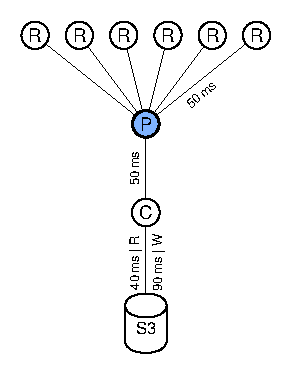
\includegraphics[width=.32\linewidth]{ps/diag-1}
        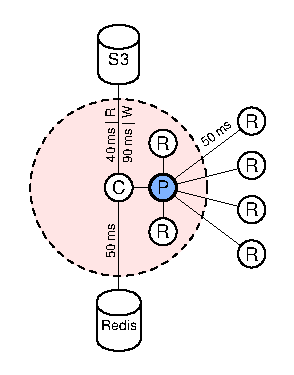
\includegraphics[width=.32\linewidth]{ps/diag-2}
        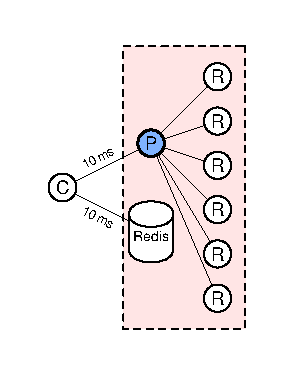
\includegraphics[width=.32\linewidth]{ps/diag-3}\\
        (a) \hspace{2.7cm} (b)
    \caption{Deployment scenarios: (a) cloud client (with either
    Redis or S3), (b) collocation center with Redis. The shaded area represents a
    LAN (or a data center). Latencies will be used in the
    evaluation (in the case of S3, $R$ represents the latency of
    reads and $W$ the latency of writes). $C$ is the client, $R$ is a replica and $P$ is the proxy replica.
    }\label{fig:deployments}
\end{figure}


To minimize the chance of correlated faults of individual metadata
servers, each replica can be at a different location, depending on the
deployment scenario. For example, the \ac{TEEMS} replicas may be
distributed over multiple administrative domains to make it less
likely that several of them can be rolled back at any given time. One
way to achieve this distribution is to colocate some replicas with a
client in a data-center, with the remaining replicas in other
administrative domains (Figure~\ref{fig:deployments}a).  In another
example scenario, clients execute on their own premises and wish to
share data items stored in the Cloud with other clients, without
trusting the Cloud. They can use \ac{TEEMS} replicas deployed at a local
collocation center, where subsets can be physically isolated and
operated by independent providers, possibly using storage in the same
center (Figure~\ref{fig:deployments}b).

Depending on their cost and availability needs, clients may opt to
store a single copy on a single cloud storage service provider,
multiple copies on independent providers, or multiple erasure coded
fragments on independent providers. In the common case, a copy or a
small set of fragments can be efficiently retrieved from the nearest
providers.


\section{Implementation}\label{sec:teems_impl}

We implemented the \ac{TEEMS} prototype in Intel SGX (version 1),
using C++. The \ac{TEEMS} servers are implemented using a
single-threaded event loop and 6KLoC (\ac{TEEMS}). Additionally,
the client library, which interacts with the replicas and with
the untrusted storage, takes up to 5KLoC (\ac{TEEMS}). We used
Flatbuffers~\cite{flatbuffers} to define our protocol messages
and their serialization, but implemented the secure transport
between the replicas using OpenSSL~\cite{openssl}.

It is important to observe that since in \ac{TEE} replicated
systems replicas cannot generally trust clients to execute the protocol
code correctly, our prototypes implement the driver code
collocated with the replicas. This means that, for instance, a
register write request is first sent to a \ac{TEEMS} server (typically, one
collocated with the client) which acts as a proxy and runs the
two rounds of the protocol. A possible alternative would have been
to implement a \ac{TEE} library that drives the register
protocol, which all replicas would remotely attest. We chose
not to do this, since the former approach has wider applicability
(e.g., it allows clients that do not run in \ac{TEE}-enabled
platforms to interact with a \ac{TEE} replicated system).

All prototypes are open-sourced under the MIT license
and available at \url{https://gitlab.mpi-sws.org/restart-rollback}.

\section{Evaluation}\label{sec:teems_eval}


We evaluate the \ac{TEEMS} prototype based on the \ac{RR} model
using benchmark workloads, aiming to answer the following questions:

\begin{enumerate}
    \item What is the overhead added by \ac{TEEMS} to secure a cloud storage system under different
      deployments?  (\S\ref{ssec:teems_eval_deploy})
    \item What is the performance of this system  when used to store
      metadata for a \ac{KVS} (Redis) under a benchmark
        workload (\ac{YCSB})?
      (\S\ref{ssec:ycsb})
\end{enumerate}

\paragraph{Experimental Setup.}
We ran our experiments using 7 machines  with
Intel$^\text{\textregistered}$ Xeon$^\text{\textregistered}$ E-2174G
processors running Debian Linux version 4.19 to run the replicas,
plus 2 machines equipped with Intel$^\text{\textregistered}$
Xeon$^\text{\textregistered}$ Platinum 8260M processors running Debian
Linux version 5.4: one of them to execute the clients and the other to
host Redis.
%
We again leveraged \texttt{sloth}~\cite{sloth} to simulate
different network topologies.

In our result graphs, each data point represents the median
measurement over $3,000$ requests and the error bars show the $5^{\text{th}}$ and
$95^{\text{th}}$ percentiles.

\begin{figure*}[t]
    \centering
    \begin{minipage}[t]{0.45\linewidth}
        \centering
        \includegraphics[width=\linewidth]{teem_results/deployment/result/client_cloud_s3}
        \caption{Client in the Cloud w/ S3}\label{fig:cloud_client_s3}
    \end{minipage}
    \begin{minipage}[t]{0.45\linewidth}
        \centering
        \includegraphics[width=\linewidth]{teem_results/deployment/result/client_cloud_redis}
        \caption{Client in the Cloud w/ Redis}\label{fig:cloud_client_remote_redis}
    \end{minipage}
    \begin{minipage}[t]{0.50\linewidth}
        \centering
        \includegraphics[width=\linewidth]{teem_results/deployment/result/collocation_center}
        \caption{Collocation Center w/ Redis}\label{fig:coloc_redis}
    \end{minipage}
    \caption{Latency in different deployment scenarios. The
    ``s3'' and ``redis'' bars refer to direct accesses to the
    untrusted storage, providing a performance baseline without
    rollback protection. ``teems'' refers to accesses without
    caching. ``teems + name cache'' and ``teems +
    blob cache'' refer to accesses where the name and blob
    caches had a hit, respectively. Caching only applies for
    get requests, and in the cases of
    Figures~\ref{fig:cloud_client_s3} and~\ref{fig:cloud_client_remote_redis}
    the ``value cache'' exists, but is close to zero since the
    cache hit with a local read quorum means there is no network
    latency access in the critical path.}
\end{figure*}



%-------------------------------------------------------------------------------
\subsection{\ac{TEEMS}-based storage}\label{ssec:teems_eval_deploy}
%-------------------------------------------------------------------------------
First, we focus on understanding the performance of our example
application, the  \ac{TEEMS}-based secure storage service, under
different deployments, which differ in the relative location of
the client, the metadata servers, and the type and location of
the untrusted storage. In this set of experiments, our baselines
are the untrusted
storage systems being used in each situation, namely Amazon S3 and an
instantiation of Redis on our local cluster, to which we optionally
add a variable  latency on the
access link.

We consider three representative deployment scenarios, illustrated in
Figure~\ref{fig:deployments}.

\paragraph{Client in the Cloud.}
In this deployment (Figure~\ref{fig:deployments}a), the client is
co-located with three metadata servers and the remaining four servers
are in another data-center.  We use two variants of storage: a
remote Redis deployment, and S3.

\paragraph{Collocation Center.}
In this scenario (Figure~\ref{fig:deployments}b), all metadata
servers and the Redis deployment are in the same collocation center, being hosted by different cloud
providers.

In both cases, the largest administrative domain has $4$
replicas, while at most $2$ replicas are expected to crash
in a correlated fashion. As such, we consider $M_R = 4$ and $F= 2$.

From Figures~\ref{fig:cloud_client_s3}--\ref{fig:coloc_redis}, we
conclude that: 1) \ac{TEEMS} performance depends heavily on the deployment
scenario (in particular on the existence of local read quorums, which
are enabled by \ac{RR}); 2) name caching is effective at masking
the overhead of accessing the metadata store; 3) blob caching, when
combined with local read quorums, allows for local reads of both data
and metadata, outperforming the baseline.


\subsection{\ac{TEEMS}-based storage running \ac{YCSB}}\label{ssec:ycsb}

Next, we compare \ac{TEEMS} with using only
Redis, on the \ac{YCSB} benchmark workloads. We deployed \ac{TEEMS} in the
Client in the Cloud setting with Redis, using name caches. We use all six core workloads
of \ac{YCSB} (A--F), which have different key distributions and read/write
ratios. The size of the objects varies between 100B and 1KB, depending
on the workload and the overall size of the database is of
1000 1KB objects.
%
The results in Figures~\ref{fig:ycsb_teems} and~\ref{fig:ycsb_redis}
show that writes incur a $2\times$ overhead, which is expected since
the Redis access must be preceded by the \ac{TEEMS} metadata access. In
contrast, reads perform comparably to the baseline, due to local
read quorums and effective usage of the cache.

\begin{figure}[t]
    \centering
    \begin{minipage}[t]{0.49\linewidth}
        \centering
        \includegraphics[width=\linewidth]{teem_results/deployment/result/ycsb_redis}
        \caption{Redis baseline}\label{fig:ycsb_redis}
    \end{minipage}
    \begin{minipage}[t]{0.49\linewidth}
        \centering
        \includegraphics[width=\linewidth]{teem_results/deployment/result/ycsb_teems}
        \caption{\ac{TEEMS} + Redis}\label{fig:ycsb_teems}
    \end{minipage}
    \caption{Latency with \ac{YCSB} workloads}
\end{figure}


\cleardoublepage{}

\fancychapter{Leveraging the \ac{RR} model in distributed storage}\label{chap:storage}
\cleardoublepage{}

In this chapter, we will present the \acf{R2-S2}, a replicated
\ac{KVS} based on LevelDB~\cite{leveldb}, a single node \ac{KVS}
implemented using  \acp{LSM-tree}~\cite{lsm}. We have developed
\ac{R2-S2} to showcase the broad applicability of the \ac{RR}
model by using it in a non-security context.

The motivation for \ac{R2-S2} is presented in
Section~\ref{sec:r2s2motivation}, followed by its design in
Section~\ref{sec:r2s2design}. We present guidelines for system
parametrization in Sections~\ref{sec:r2s2parametrization}.
Section~\ref{sec:r2s2implementation} describes the implementation
of the PoC and a preliminary evaluation is presented in
Section~\ref{sec:r2s2evaluation}.

\section{Motivation}\label{sec:r2s2motivation}
Batching multiple small write operations to a block-oriented storage device into a
single large one is a known mechanism to increase its throughput.
To achieve this batching, one has to wait for an adequate amount
of contiguous data to write, which introduces a delay in the
operation. Alternatively, once the data to write is present in
an in-memory buffer (soft state) the system could return to the
client. This opens the possibility of data loss, if the system
crashes before effectively synchronizing this data to the persistent
storage device.

% 5: replication should be able to partially mask this
%
% note: we can introduce the difference between persistent replicated
% storage systems and volatile replicated storage systems
This problem is propagated as is to current persistent replicated storage
systems: the throughput of the system is limited by the
throughput of the storage devices of the replicas. To avoid this
performance penalty, some replicated systems consider data to be persisted if it is
present in volatile memory at a sufficiently large subset of replicas~\cite{pbft}
(i.e., persistence through replication). Such an approach is not
consensual, with other authors insisting that data must be
present in stable storage to be considered
persisted~\cite{bolosky:paxos}.

% Question whether this needs to be a dichotomy
We argue that these two properties --- performance and
durability --- do not need to be mutually exclusive. Instead, we
aim to combine both into a system that offers the throughput from
the solutions that persist in the background with the high
durability from systems that persist before replying to
requests.

% We present a new replication strategy
To this end, we present a novel replication strategy based on
carefully and strategically mixing both approaches, leveraging
\ac{RR} quorum systems. Instead of issuing the write
requests simmetrically to all replicas, as is costumary, we can
strategically signal to certain replicas to synchronize to
persistent storage before replying while allowing others to
acknowledge the write eagerly, thus mixing both approaches. This
key insight allows us to take advantage of batching, improving the overall
performance of the system, without relinquishing fault tolerance.
The \ac{RR} fault model is needed in case replicas crash before
synchronizing their soft state to stable storage.

% 8, 9: challenges
This approach opens a series of challenges. The storage layer
requires careful adaptations to support multiple modes of
operation while offering efficient batching, even on
non-sequential writes. At the replication level, the asymmetry of
operation between replicas introduces the problem of \emph{sync
scheduling}: choosing which replicas synchronize to persistent storage
and which can reply eagerly. This schedule is paramount to
extracting the maximum performance of the system, and offers a
rich design space. Parametrizing a deployment of such a system is
also not obvious. There is a tradeoff to be explored between the
total number of replicas, the number of replicas that synchronize
to disk in the background (and, by extension, the performance of
the system) and the desired availability and reliability of the
system. We present a principled method for this parametrization,
where a system administrator can tune the number of replicas
based on how prone to faults they are and the desired
availability and durability levels.

%%%%%%%%%%%%%%%%%%%%%%%%%%%%%%%%%%%%%%%%%%%%%%
\section{\ac{R2-S2} Design}\label{sec:r2s2design}
%%%%%%%%%%%%%%%%%%%%%%%%%%%%%%%%%%%%%%%%%%%%%%

This section presents the design of \ac{R2-S2}
based on the principle of \emph{asymmetric synchronization}. However,
before discussing our architecture in detail, it is worthwhile to
categorize in a systematic way the three approaches that can be used to synchronize
replica state to stable storage.

\paragraph{Sync immediately.} When receiving an object to write, a
replica immediately writes and flushes the object to stable
storage, issuing the reply afterwards. This prevents batching,
which favours \emph{durability} and \emph{latency} in detriment
of \emph{throughput}.

\paragraph{Batch and wait.} When receiving an object to write, a
replica places the object in a batch and waits for this batch to
be flushed to stable storage. Afterwards, the reply can be
issued. Since there is batching and objects are being persisted
before replying, this approach favours \emph{durability} and
\emph{throughput} at the cost of \emph{latency} (which can be
very large if the batch takes a long time to be filled due to a
lack of writes).

\paragraph{Batch and reply (Move fast and break things).} In this approach,
replicas place the object in the batch (i.e., volatile memory)
and reply immediately. This achieves the best \emph{latency} and
\emph{throughput}, sacrificing \emph{durability} since replicas
can suffer a rollback if they crash and restart.

The state of the art seems to hint at
an impossibility trinity: systems have to pick two between latency,
throughput, and durability. The design goals of \ac{R2-S2} aim to question this
impossibility, by showing that there can be interesting
combinations of these features that, at least, approximate the
best of the three approaches:
\ac{R2-S2}:
\begin{enumerate}
    \item \textbf{Strong Persistence}: data loss should never
        ocurr, even in the presence of arbitrary node crashes;

    \item \textbf{Performance}: the architecture should yield
        performance gains compared to
        Approaches A and B\@;
\if 0
    \item \textbf{Generality}: the architecture should be as
        generic as possible. In particular, it should be
        applicable to a variety of replication protocols.
\fi
\end{enumerate}

Note that none of our baselines satisfy all requirements:
approaches A and B achieve
\emph{strong persistence} but not the performance requirement.
Approach C does meet the performance
requirement, but does not satisfy \emph{strong persistence}.

In the remainder of this section, we will describe
\emph{asymmetric synchronization}, the key technique that realizes the
goals prescribed above, and how the architecture needs to
acommodate this paradigm to achieve the best possible
performance.

%%%%%%%%%%%%%%%%%%%%%%%%%%%%%%%%%%%%%%%%%%%%%%
\subsection{Asymmetric Synchronization}\label{ssec:asymmetric_synchronization}
%%%%%%%%%%%%%%%%%%%%%%%%%%%%%%%%%%%%%%%%%%%%%%

Asymmetric synchronization is the key to extracting performance
in \ac{R2-S2}. The core idea is to partition the replica set
into two disjoint subsets: the \emph{volatile set}
$\mathbbm{R}$, composed of the replicas that eagerly reply to the
request before synchronizing to persistent storage (and thus can
suffer a rollback on restart); and the sync set $\mathbb{F}$,
comprised by the
replicas that wait until the data is persisted before replying.
When issuing a write request, each replica is told in which set
they belong to, and act accordingly. An important subset of
$\mathbb{F}$ is its intersection with the write quorum
$\mathbb{W}_Q$. This subset is comprised by the replicas that are
critical to the performance of the write operation (in
particular, its latency) and is referred as the \emph{critical
sync set} from now on.

\paragraph{Achieving strong persistence.} To achieve strong
persistence, it is sufficient that the critical sync set is
never null. This implies that there is always at least one
replica in every write quorum which persisted the value, making
it recoverable. This is guaranteed by the \ac{RR} quorum
system, by setting the maximum size of $\mathbbm{R}$ to $M_R$,
since the volatile replicas are the ones which can suffer the rollback on
restart.

\paragraph{Improving performance.}The key to improving throughput
(compared to approach A) is scheduling. Intuitively, it is
this will distribute the burden of syncing to disk among the
replica set, allowing all the replicas to batch eventually. By
having all replicas reply as soon as possible we also get a
latency improvement compared to approach B. Regretablly, although
this approach does yield performance benefits compared to
approaches A and B, it is impossible to match the performance of
C\@: this would require removing any synchronizing writes from the
critical path, making $\mathbb{W}_Q \cap \mathbb{F} =
\varnothing$, violating strong persistence.

\rr{The last three paragraphs have really poor cohesion. They are
three separate and seemlingly unrelated ideas, which makes for a
very difficult read. You should expand and rethink the
structure}\bsd{tried to connect it better, but discuss}

\new{
%%%%%%%%%%%%%%%%%%%%%%%%%%%%%%%%%%%%%%%%%%%%%%
\subsection{System Overview}\label{ssec:r2s2overview}
%%%%%%%%%%%%%%%%%%%%%%%%%%%%%%%%%%%%%%%%%%%%%%

\begin{figure}[t]
    \centering
    \includegraphics[width=\linewidth]{img/r2s2_arch}
    \caption{Architecture of the \ac{R2-S2}
    prototype}\label{fig:r2s2arch}
\end{figure}

The \ac{R2-S2} system is comprised of a client and several
servers, where the client is implemented as a library that
implements the replication layer and handles the connection to
and coordination of the multiple \ac{R2-S2} servers.

Each \ac{R2-S2} server consists of an RPC controller, which
handles the interface with the client. This controller manages
the server's local \ac{KVS} (in our case,
LevelDB~\cite{leveldb}). In our prototype, we chose to implement
the ABD~\cite{abd} protocol, since its read/write interface
maches perfectly with the \ac{KVS} interface we are aiming to
implmenet. One relevant aspect of ABD, and most other replication
protocols, is the notion of object versions, which are not directly supported by the
\acp{KVS}. To order concurrent writes to the same object with
different timestamps, an in memory timestamp cache is required. This
cache is populated as needed, with synchronization on the values
to order the writes to ensure that a newer value is not
overwritten by a previous one.

The overall architecture of the \ac{R2-S2} prototype is
summarized in Figure~\ref{fig:r2s2arch}.

}

%%%%%%%%%%%%%%%%%%%%%%%%%%%%%%%%%%%%%%%%%%%%%%
\subsection{Scheduling}\label{ssec:schedule}
%%%%%%%%%%%%%%%%%%%%%%%%%%%%%%%%%%%%%%%%%%%%%%

As we have covered, a good schedule is crucial to realize the
performance potential of the architecture. A \emph{schedule} is a
sequence $S$, where $S_i^j$ is the mode of operation (batch and
reply, batch and wait or sync to log) to be applied by replica
$i$ for the $j^\text{th}$ write operation. The
schedule is said to be \emph{valid} if the volatile set (i.e,
the number of batch and reply modes of operation) does not exceed
$M_R$, for every $S^j$. Thus, any valid schedule guarantees
strong persistence.

There are several approaches to scheduling. Which is preferable
is non-obvious beforehand: the schedule will be sensitive to the
particularities of the replication protocol, the deployment and
the operation load. In the preliminary evaluation in
\S~\ref{sec:r2s2evaluation} we present an
evaluation of some of the scheduling policies described
here.

At a high level, there are two types of schedules: \emph{static}
schedules, which can pre-determined ahead of time, and as such
are independent of the load the system is being subjected to; and
\emph{dynamic} schedules, which are computed on the fly and as
such can be \emph{reactive} to the load and current status of the
system. In this dissertation we will focus on static schedules,
as they are simpler and sufficient to showcase the gains from the
\ac{RR} model.

\paragraph{Constant Schedule.} A constant schedule is one where
all write operations use the same modes of operation for each
replica. In other words, all $S^j$s are equal. This schedule is,
at face value, a poor choice, since it prevents the replicas in the
critical set from ever batching. However, if the replica set is
very heterogeneous, this might be used to provide a tailored
approach to the hardware characteristics.

\paragraph{Random Schedule.} A schedule where replicas are
randomly allocated to the sync and volatile sets (based on the
sizes they need to have for the schedule to be valid).

\paragraph{Round Robin Schedule.} A schedule where the sync set
is shifted at each round. For instance, in a system with $N = 5,
M_R = 2$, replicas $0, 1, 2$ are the sync set at step $j$, and
at step $j + 1$ replicas $3, 4, 0$ become the sync set, and so
on.

\bsd{TODO: figures with schedule time diagrams}

Assuming a good random number generator, both the random and the
round robin schedules should evenly distribute the load among the
replicas. However, the random scheduler may offer less
predictable performance.

%%%%%%%%%%%%%%%%%%%%%%%%%%%%%%%%%%%%%%%%%%%%%%
\subsection{Storage Layer}\label{ssec:storage}
%%%%%%%%%%%%%%%%%%%%%%%%%%%%%%%%%%%%%%%%%%%%%%

The storage layer plays a crucial role in realizing the
performance potential of the system. It needs to efficiently support
three different types of write operations, one for each of the
different baseline approaches. It will also need to support read operations
efficiently. Figure~\ref{fig:storage_layer} shows a diagram of
the storage layer and its data-structures.

An \ac{LSM-tree} is employed as the core data structure of the storage
layer, enabling the sequential writes required for batching as
well as providing reasonable read performance. There exists a
log, used to write values that need to be synced immediately, and
an in-memory batch for values that should be batched. To further speed
up reads there is an optional in-memory object cache.

\begin{figure}[t]
    \centering
    \includegraphics[width=.75\linewidth]{img/storage_layer}
    \caption{Diagram of the Storage Layer}\label{fig:storage_layer}
\end{figure}


There is an additional in-memory cache, which only stores the
object versions. This is useful because versions are a staple of
most replication protocols and several of them require reading
the current version before writing a new one. Since versions are
constant-sized and small, the capacity of the version cache can
be significantly larger than that of the object cache. This cache
is required to synchronize concurrent writes of different
versions to the same key. When the node is writing a value, it required to
check the version cache, populating it if required, where an
atomic update is executed on the version to ensure that an old
version does not override a newer version it is racing with.

With these data structures in place, the various operations
requried to implement the \ac{KVS} interface and asymmetric
syncing become quite simple. Satisfying version reads is simple:
the timestamp cache is consulted (falling back on the
\ac{LSM-tree} and log if needed). The workflow of an object read
is similar: if the object cache exists it is consulted, falling
back on the \ac{LSM-tree} and the log in the event of a miss.
Handling batch and reply writes requires placing the value
in the batch and eventually a background thread will flush the
batch into the \ac{LSM-tree}. Handling sync and reply writes
amounts to placing it in the persistent log, with this log being
compacted into the \ac{LSM-tree} at a later time by a background
thread.


%%%%%%%%%%%%%%%%%%%%%%%%%%%%%%%%%%%%%%%%%%%%%%
\section{Parametrizing the System}\label{sec:r2s2parametrization}
%%%%%%%%%%%%%%%%%%%%%%%%%%%%%%%%%%%%%%%%%%%%%%

To parametrize our system, we effectively need to choose
appropriate values for $M_R$ and $F$. We employ a data-driven
approach to this problem. Relying on real-world information about
the availability and reliability of components, we can predict
the reliability and availability of the system as a function of
$M_R$ and $F$. Choosing the adequate values becomes an exercise of
setting the desired reliability/availability and solving for $M_R$
and $F$.

The availability of the system (probability that it is available
at a particular point in time) is impacted by the availability of
the individual replicas. Let $p_c$ be the symmetric of the
availability of a replica, ie: the probability that a replica is
\emph{crashed} at a particular point in time.

The reliability (probability that the system loses data over a
given period of time) of the
system is dependent on the reliability of the underlying storage
devices and the availability of the replicas in the eager set.
Let $p_f$ be the probability that a storage device fails
(irrecoverably) in that period of time.

\new{
In order to derive the parametrization of the system, let us
begin with a simplifying assumption that all failures (both
crashes and storage device failures) are independent among all
replicas, an assumption valid for a geo-replicated deployment,
for instance. Let us first consider reliability. The probability
that all replicas in the eager set crash (and thus all the
replicas that only had the data in volatile storage lose that
data) is $p_c^{M_R}$, since $M_R$ is the size of the eager set.
To truly lose the data, the remainder of the replicas in the
write quorum would have had to suffer an irrecoverable fault in
their storage devices, which happens with probability $p^{W_Q -
M_R}$. Due to the independence of failures, we can derive the
probability that data is lost to be $p_c^{M_R} \cdot p_f^{W_Q -
M_R}$, making the reliability of the system be $1 - p_c^{M_R}
\cdot p_f^{W_Q - M_R}$. Considering availability, we know that
the system is available if a read quorum and a write quorum are
available. Due to the independence of failures, the quorums
become unavailable with probability $p_c^{R_Q}$ and $p_c^{W_Q}$,
repectively. As such, the probability that they are both
available at a given point in time is simply $1 - p_c^{\min(R_Q,
W_Q)}$.

Now let us imagine that the probability of replicas crashing
\emph{is} correlated, as is the case in a datacenter deployment.
Then, the probability of $n$ replicas crashing is the same as the
probability of a single replica crashing: $p_c$. Considering
reliability, this means that the probability of the eager set
losing its volatile state due to a crash \emph{and} the remainder
of the write quorum suffering an irrecoverable failure is $p_c
\cdot p_f^{W_Q - M_R}$. Availability is quite simpler to derive,
as if the probability of quorums of any type being unavailable is
simply $p_c$, making the availability of the system $1 - p_c$.
}


Table~\ref{tab:parametrization} summarizes the availability and
reliability of the system in these two scenarios.

\begin{table}[ht]
    \centering
    \caption{Availability and reliability in a geo-replicated
    deployment versus a datacenter deployment. $R_Q$ and $W_Q$
    are the sizes of the quorums for a parametrization with $M_R$
    tolerated rollbacks and $F$ crash faults}\label{tab:parametrization}
    \begin{tabular}{|r||c|c|}
        \hline
        & \textbf{Geo-replicated} & \textbf{Datacenter} \\ \hline
        \textbf{Availability} & $1 - p_c^{\min(R_Q, W_Q)}$ & $1 - p_c$ \\ \hline
        \textbf{Reliability}  & $1 - p_c^{M_R} \cdot p_f^{W_Q - M_R}$ & $1 - p_c \cdot p_f^{W_Q - M_R}$ \\ \hline
    \end{tabular}\label{tab:parametrization}
\end{table}



%%%%%%%%%%%%%%%%%%%%%%%%%%%%%%%%%%%%%%%%%%%%%%
\section{Preliminary Evaluation}\label{sec:r2s2evaluation}
%%%%%%%%%%%%%%%%%%%%%%%%%%%%%%%%%%%%%%%%%%%%%%

In this section, we present our preliminary evaluation of the
\ac{R2-S2} prototype. We aim to answer two fundamental questions
about the approach:

\begin{enumerate}
    \item What performance benefits can be extracted using
        \emph{asymmetric synchronization}?
        (\S\ref{ssec:r2s2_eval_asym})
    \item What is the impact of different schedules in the
        performance of the \ac{R2-S2} system?
        (\S\ref{ssec:r2s2_eval_scheduling})
\end{enumerate}

%%%%%%%%%%%%%%%%%%%%%%%%%%%%%%%%%%%%%%%%%%%%%%
\subsection{Implementation}\label{sec:r2s2implementation}
%%%%%%%%%%%%%%%%%%%%%%%%%%%%%%%%%%%%%%%%%%%%%%

We implemented \ac{R2-S2} using LevelDB~\cite{leveldb} as the
underlying storage layer and our own replication layer on top of
it. This was extremely helpful since LevelDB already implements
the \ac{LSM-tree}, the persistent log and the optional object cache
out of the box, and provides for two out of the three modes of
operation: \emph{batch and reply} and \emph{sync and reply}.
\new{We intend to implement the \emph{batch and wait} mode of
operation and incorporate it in our prototype. However, this
requires changing LevelDB to track the batches each object is
placed in and when those batches are eventually persisted.}

The replication layer was implemented in Rust with the request transport
being handled by gRPC~\cite{grpc}. The \ac{R2-S2} client library
provides a shim that interacts with the replication layer that
coordinates the \ac{ABD} operations. The \ac{R2-S2} server
receives requests via gRPC and manages the timestamp cache and
its embedded LevelDB instance.

The client library was implemented in approximately 2KLoC of
Rust. The server was implemented in 400LoC. The gRPC protocol
definition is comprised of 135 LoC. All the remainder driver code
for benchmarks consists of 2KLoC of Rust.

%%%%%%%%%%%%%%%%%%%%%%%%%%%%%%%%%%%%%%%%%%%%%%
\subsection{Methodology}\label{ssec:r2s2methodology}
%%%%%%%%%%%%%%%%%%%%%%%%%%%%%%%%%%%%%%%%%%%%%%

\begin{figure}[t]
    \centering
    \includegraphics[width=.75\linewidth]{r2s2_results/abd_small/tput.pdf}
    \caption{Maximum throughput for different configurations.
    The \emph{batch and reply} configuration places the
    object in a batch and replies immediately, while in the \emph{sync and reply} configuration all replicas
    flush the object to the persistent log before replying. In
    the $T(BR, 5)$, $BR$ replicas in each write use the former
    approach, while the remaining use the
    latter.}\label{fig:r2s2_asym}
\end{figure}
\paragraph{Experimental Setup.}
We ran our experiments using 5 machines  with
Intel$^\text{\textregistered}$ Xeon$^\text{\textregistered}$ E-2174G
processors running Debian Linux version 4.19 with \bsd{TODO:
insert specification of the HDD} to run the replicas,
plus one machine equipped with a Intel$^\text{\textregistered}$
Xeon$^\text{\textregistered}$ Platinum 8260M processor running Debian
Linux version 5.4 to execute the client driver of the benchmarks.

\paragraph{Experimental Methodology.} In our result graphs, each data point represents the average
measurement throughput measurement over $60$ seconds of running
at load, using an open-loop client (i.e., a client that issues a
request asynchronously at regular time intervals to achieve the
desired load). To find the throughput in each configuration, we
ran the experiment with multiple offered loads to find the
maximum throughput point.


%%%%%%%%%%%%%%%%%%%%%%%%%%%%%%%%%%%%%%%%%%%%%%
\subsection{Asymmetric
Synchronization}\label{ssec:r2s2_eval_asym}
%%%%%%%%%%%%%%%%%%%%%%%%%%%%%%%%%%%%%%%%%%%%%%

In this experiment, we compare two baselines in the classical
\ac{CFT} model, \emph{sync and
reply} and \emph{batch and reply}, with a set of \emph{threshold
configurations} ($T(BR, N)$), which vary the number of replicas that use the
batch and reply synchronization mode. Effectively, $T(0, N)$ is
the \ac{CFT} sync and reply configuration and $T(N, N)$ is the
\ac{CFT} batch and reply configuration.

We measured the maximum throughput of each configuration using a
randomized schedule and $128KB$ objects. As we can observe in
Figure~\ref{fig:r2s2_asym}, the more replicas are
allowed to batch the higher the average throughput.


%%%%%%%%%%%%%%%%%%%%%%%%%%%%%%%%%%%%%%%%%%%%%%
\subsection{Scheduling}\label{ssec:r2s2_eval_scheduling}
%%%%%%%%%%%%%%%%%%%%%%%%%%%%%%%%%%%%%%%%%%%%%%

\bsd{THE INTERPRETATION IS IS TOTALLY WRONG}

Next, we compare the same two baselines in the
\ac{CFT} model, \emph{sync and
reply} and \emph{batch and reply} with three \ac{RR} based quorum
configuration which aim to combine the durability of the former and
performance of the latter. Each of the \ac{RR} configurations
uses a different static schedule, as described in
Section~\ref{ssec:schedule}: constant, random and round robin.
These configurations have $M_R = 2$ and $F = 2$. This matches
both the number of tolerated crash faults of the \ac{CFT}
baselines and the total number of replicas.


\begin{figure}[t]
    \centering
    \includegraphics[width=.75\linewidth]{r2s2_results/rr_small/tput.pdf}
    \caption{Maximum throughput for different schedules.
    The \emph{batch and reply} configuration places the
    object in a batch and replies immediately, while in the \emph{sync and reply} configuration all replicas
    flush the object to the persistent log before replying. The
    constant schedule always synchronizes to the same $3$ of the
    $5$ replicas. The randomized schedule also synchronizes to
    $3$ replicas, but these get randomized every operation. The
    round robin schedule changes the $3$ replicas at each
    operation in a cycle.}\label{fig:r2s2_sched}
\end{figure}

We measured the maximum throughput of each configuration using  $128KB$ objects.
As we can observe in Figure~\ref{fig:r2s2_sched}, both the random
and the round robin schedules achieve a middle ground between the
performance of the \emph{sync and reply} and \emph{batch and
reply} configurations, while still achieving strong persistence.
The constant schedule shows comparable performance to the
\emph{sync and reply}. This is because the performance of a
quorum operation is limited by the slowest replica in the quorum.
Since having a replica in the quorum that synchronizes before replying is a
pre-requisite to strong persistence and in the constant schedule
the replicas that synchronize never get to batch, the load is
unevely distributed. This causes the throughput to be severly
limited.


\cleardoublepage{}

\fancychapter{Conclusions and Future Work}\label{chap:conclusion}
\cleardoublepage{}

In this dissertation, we have presented the \acf{RR} fault model,
designed for replicated \acp{TEE} with external state. We have
provided an extensive formalization of the model, resulting
quorum systems and its properties, and laid out guidelines for
adapting existing \ac{CFT} protocols to the model with little
effort. We have furthermore experimentally verified that these
resulting protocols are on par in terms of performance with their
\ac{CFT} counterparts (which do not provide safety in the case of
replicated \acp{TEE} with persistent state) and significantly
outperform the \ac{BFT} counterparts that would otherwise be
required to tolerate rollback faults.

We have shown the general applicability of this model, both in
\ac{TEEMS} and \ac{R2-S2}. In \ac{TEEMS}, we have designed and
implemented a metadata service that can be used to enhance
existing cloud storage systems with \ac{TEE}-grade security. Our
evaluation of \ac{TEEMS} shows that the overhead it incurs is
modest. In \ac{R2-S2}, we have shown the potential of this fault
model outside the \ac{TEE} use case, by designing a distributed
\ac{KVS} that strikes a balance between performance and
durability, which would otherwise be impossible in the \ac{CFT} model. Our
preliminary evaluation of \ac{R2-S2} shows that there are
performance gains in using the \ac{RR} model, compared to simply
synchronizing to all replicas.

In the future, we aim to refine the \ac{R2-S2} prototype, showing
its applicability in other replication protocols other than
\ac{ABD}. We also wish to modify LevelDB to be able to
implement the \emph{batch and wait} semantics, and further
improve the performance of the system. Additionally, we aim to
conduct a survey on frequency of failures (both crash faults and
disk corruptions) that would help us instantiate the
parameterizations described in
Section~\ref{sec:r2s2parameterization} with real world data.
Another high level forward looking vision is to study the
possible benefits and limitations of conceptually separating a
node's computation (code and volatile memory) and its persistent
state. This approach would not only provide an interesting
description of the \ac{RR} model but also have wider
applicability, for instance in the context of network connected
disks that can be used by multiple nodes.

\cleardoublepage{}

% BIBLIOGRAPHY
\pdfbookmark[0]{Bibliography}{bib}
\addcontentsline{toc}{chapter}{Bibliography}
\bibliographystyle{IEEEtran}
\normalem{}
\bibliography{main}

% The following command modifies the 'emphasis' style for bibliography entries
\ULforem{}
\cleardoublepage{}

%\printglossary[]
\mtcaddchapter{}

\cleardoublepage{}

\appendix
\pdfbookmark[1]{Appendix A}{appendix}
% #############################################################################
% This is Appendix A
% !TEX root = ../main.tex
% #############################################################################
\chapter{An Appendix}
\label{chapter:appendixA}


\cleardoublepage{}

%\pdfbookmark[1]{Appendix B}{appendix}
%% #############################################################################
% This is Appendix B
% !TEX root = ../main.tex
% #############################################################################
\chapter{Another Appendix}
\label{chapter:appendixB}

%\cleardoublepage{}

\end{document}
